\documentclass[11pt]{article}
\usepackage[margin=1in]{geometry}
\usepackage{graphicx}
\usepackage{booktabs}
\usepackage{hyperref}
\hypersetup{colorlinks=true,linkcolor=blue,urlcolor=blue}
\title{Episode Mini-Backtest Report}
\author{TP2 SPY Call Pipeline}
\date{June 2026}
\begin{document}
\maketitle

\section*{Purpose}
The episode mini-backtest assigns strategy-level realized P\&L labels to each
episode start. It is a labeling layer for later ML, not a final trading system.
Rows with invalid or unobservable exits are retained and counted instead of
being silently dropped.

\section*{Backtest Convention}
\begin{itemize}
  \item Enter the strategy at the episode start using bid/ask execution.
  \item Exit only after a clean true TP2 reversion, using exit-day bid/ask.
  \item Charge \$0.65 per option-contract side.
  \item Track T1, T2, K1, and K2 as the active strategy families.
\end{itemize}

\section*{Broad Mid-Detected Results}
\begin{center}
\begin{tabular}{lrrrr}
\toprule
Strategy & Candidates & Valid rows & Valid share & Net P\&L \\
\midrule
K1 & 2,098,213 & 1,062,589 & 50.64\% & -\$1,290.32M \\
K2 & 2,098,213 & 1,038,626 & 49.50\% & -\$1,508.97M \\
T1 & 2,098,213 & 1,038,626 & 49.50\% & -\$1,093.80M \\
T2 & 2,098,213 & 1,062,589 & 50.64\% & -\$1,708.55M \\
\bottomrule
\end{tabular}
\end{center}

\begin{figure}[h]
\centering
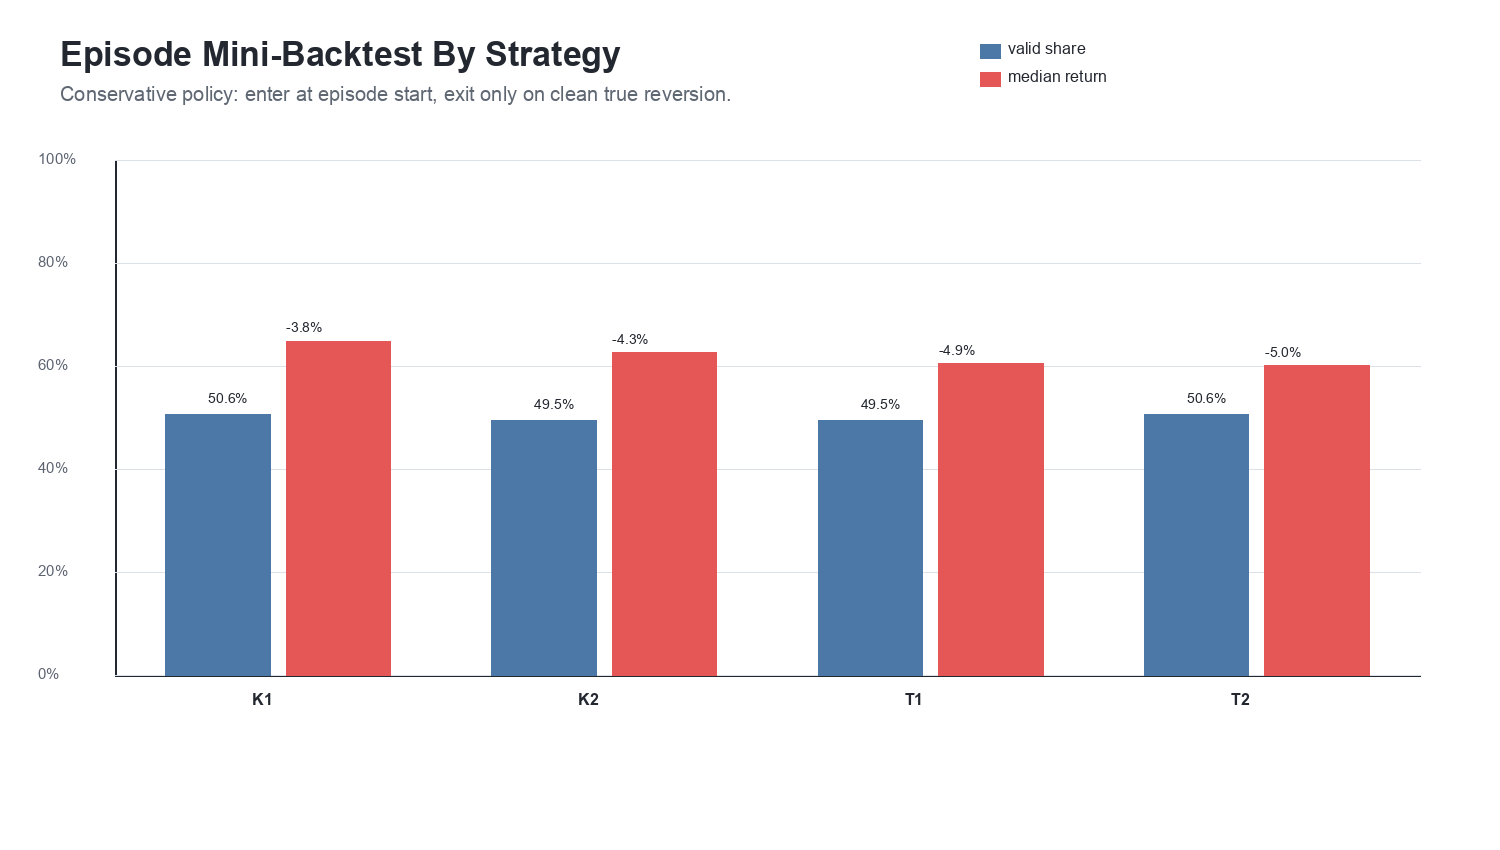
\includegraphics[width=\linewidth]{figures/episode_mini_backtest_by_strategy.png}
\caption{Valid share and median return by strategy for the broad mid-detected universe.}
\end{figure}

\begin{figure}[h]
\centering
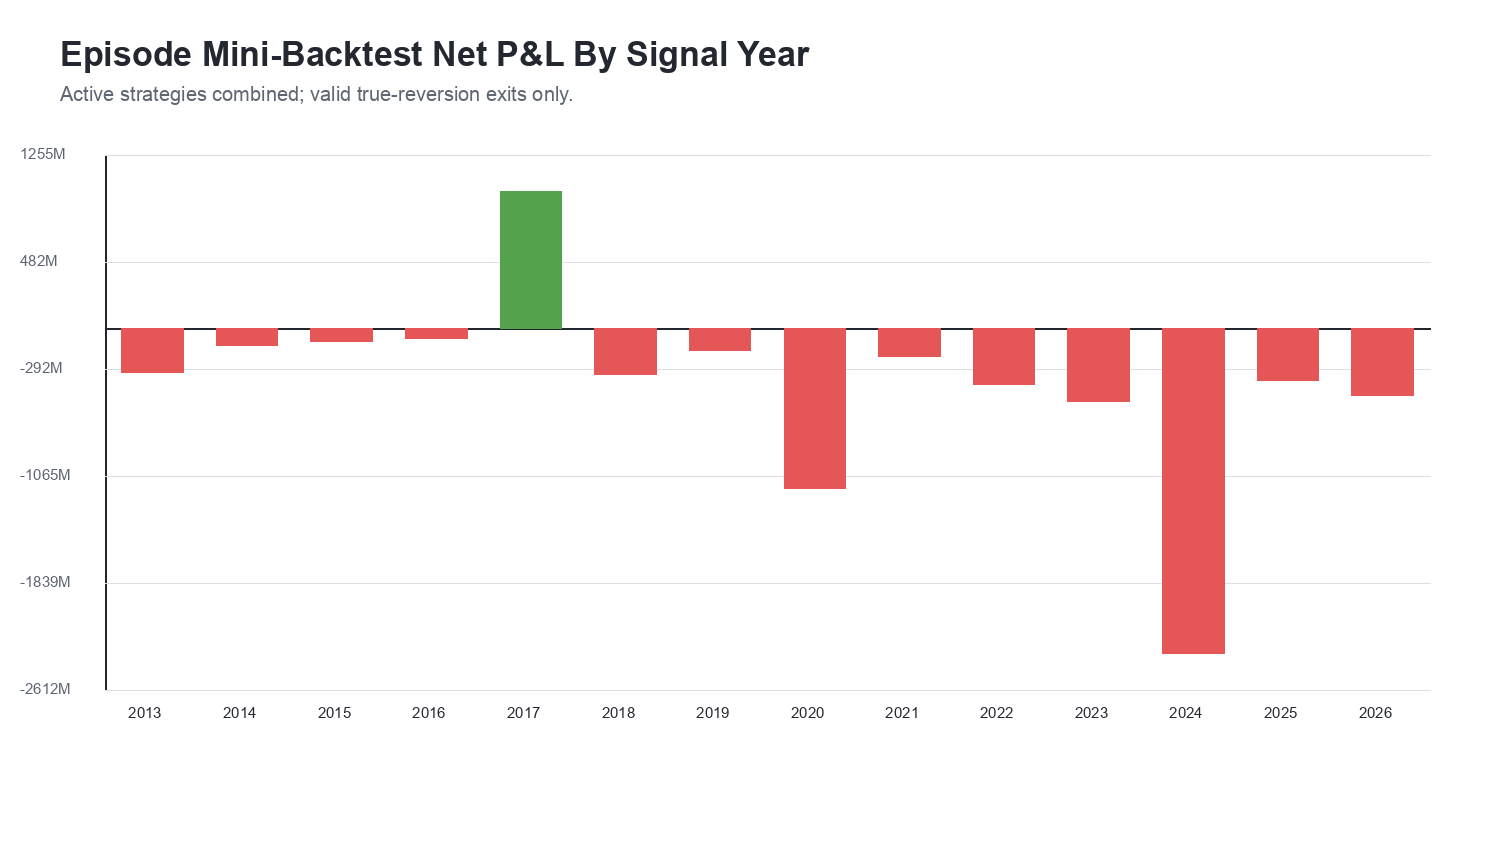
\includegraphics[width=\linewidth]{figures/episode_mini_backtest_yearly_net_pnl.png}
\caption{Broad mini-backtest net P\&L by signal year.}
\end{figure}

\section*{Interpretation}
The broad mid-detected universe is strongly negative after bid/ask execution.
That result motivated the conservative bid/ask subset, liquid-exit rebuild,
and later market-quality ML robustness checks.

\end{document}
